% !TEX TS-program = pdflatex
% !TEX encoding = UTF-8 Unicode

% This is a simple template for a LaTeX document using the "article" class.
% See "book", "report", "letter" for other types of document.

\documentclass[11pt,listof=totoc]{scrreprt} % use larger type; default would be 10pt

\usepackage[utf8]{inputenc} % set input encoding (not needed with XeLaTeX)
\usepackage{german}

%%% Examples of Article customizations
% These packages are optional, depending whether you want the features they provide.
% See the LaTeX Companion or other references for full information.

%%% PAGE DIMENSIONS
\usepackage{geometry} % to change the page dimensions
\geometry{a4paper} % or letterpaper (US) or a5paper or....
% \geometry{margin=2in} % for example, change the margins to 2 inches all round
% \geometry{landscape} % set up the page for landscape
%   read geometry.pdf for detailed page layout information

\usepackage{graphicx} % support the \includegraphics command and options
\usepackage{url}

% \usepackage[parfill]{parskip} % Activate to begin paragraphs with an empty line rather than an indent

%%% PACKAGES
\usepackage{booktabs} % for much better looking tables
\usepackage{array} % for better arrays (eg matrices) in maths
\usepackage{paralist} % very flexible & customisable lists (eg. enumerate/itemize, etc.)
\usepackage{verbatim} % adds environment for commenting out blocks of text & for better verbatim
\usepackage{subfig} % make it possible to include more than one captioned figure/table in a single float
% These packages are all incorporated in the memoir class to one degree or another...

%%% HEADERS & FOOTERS
\usepackage{fancyhdr} % This should be set AFTER setting up the page geometry
\pagestyle{fancy} % options: empty , plain , fancy
\renewcommand{\headrulewidth}{0pt} % customise the layout...
\lhead{}\chead{}\rhead{}
\lfoot{}\cfoot{\thepage}\rfoot{}

%%% SECTION TITLE APPEARANCE
\usepackage{sectsty}
\allsectionsfont{\sffamily\mdseries\upshape} % (See the fntguide.pdf for font help)
% (This matches ConTeXt defaults)

%%% ToC (table of contents) APPEARANCE
\usepackage[nottoc,notlof,notlot]{tocbibind} % Put the bibliography in the ToC
\usepackage[titles,subfigure]{tocloft} % Alter the style of the Table of Contents
\renewcommand{\cftsecfont}{\rmfamily\mdseries\upshape}
\renewcommand{\cftsecpagefont}{\rmfamily\mdseries\upshape} % No bold!

\usepackage{amsthm}
\usepackage{listings}

\usepackage{listings}
\usepackage{color}
\definecolor{lightgray}{rgb}{.9,.9,.9}
\definecolor{darkgray}{rgb}{.4,.4,.4}
\definecolor{purple}{rgb}{0.65, 0.12, 0.82}
\definecolor{gray}{rgb}{0.4,0.4,0.4}
\definecolor{darkblue}{rgb}{0.0,0.0,0.6}
\definecolor{cyan}{rgb}{0.0,0.6,0.6}

\lstdefinelanguage{XML}
{
  morestring=[b]",
  morestring=[s]{>}{<},
  morecomment=[s]{<?}{?>},
  stringstyle=\color{black},
  identifierstyle=\color{darkblue},
  keywordstyle=\color{cyan},
  morekeywords={xmlns,version,type}% list your attributes here
}

\lstset{
   language=XML,
   backgroundcolor=\color{lightgray},
   extendedchars=true,
   basicstyle=\footnotesize\ttfamily,
   showstringspaces=false,
   showspaces=false,
   numbers=left,
   numberstyle=\footnotesize,
   numbersep=9pt,
   tabsize=2,
   breaklines=true,
   showtabs=false,
   captionpos=b
}

\theoremstyle{definition}
\newtheorem{definition}{Definition}


%%% END Article customizations

%%% The "real" document content comes below...

\title{IT Service Management: End-to-end-Überwachung}
\author{Florian Lüthi}
%\date{} % Activate to display a given date or no date (if empty),
         % otherwise the current date is printed 

\begin{document}
\maketitle

\tableofcontents

\chapter{Management Summary}

\chapter{Einführung}

\section{Kontext und Definitionen}

\begin{definition}[Business Service Management (BSM)]
Das Modell des Business Service Management verknüpft die Geschäftsprozesse eines Unternehmens mit den darunterliegenden IT-Services. Dadurch ist es möglich, die Abhängigkeiten von Business zu IT darzustellen, sowie die Auswirkungen von IT-Störungen auf das Business aufzuzeigen. Das Ziel von Business Service Management ist, eine bessere Abstimmung zwischen Business und IT zu erzielen. \cite{wiki:bsm}
\end{definition}

BSM startete ungefähr im Jahr 2003 als Buzzword, bis sich Forrester Research 2006 dem Thema annahm und begann, darüber zu publizieren. \cite{wiki:bsm, forrester:bsm, forrester:implementingBsm}

\begin{definition}[End-to-End-Monitoring]
Bla,.
\end{definition}

\section{Fragestellungen}

\subsection{Transparenz versus Transformabilität}

\subsection{Skalierbarkeit nach unten}

\chapter{Lösungsansätze}

\section{Service Level Agreements (SLAs)}
Eine allgemein bekannte Definition sagt:
\begin{quote}
Ein Service Level Agreement (SLA) ist der Teil eines Dienstleistungsvertrags, in welchem die Dienstleistung formal definiert ist. In der Praxis wird der Begriff {\em SLA} manchmal für die vertraglich zugesicherte Lieferzeit verwendet. \cite{wiki:sla}
\end{quote}

Es ist offensichtlich, dass diese Definition noch nicht enorm hilfreich ist. Forrester definiert darum zwei neue Begriffe, wobei Abbildung \ref{forr} die jeweilige Abgrenzung zueinander zeigt:

\begin{definition}[Business service management (BSM)] Business service management is an intelligence layer that supports all the management processes involved in monitoring service delivery\footnote{Da sich die beiden englischen Begriffe {\em intelligence} und {\em delivery} nicht so ins Deutsche übersetzen lassen, dass der Sinn des Satzes gewahrt bleibt, wurde vom Autor auf die Übersetzung verzichtet.} \cite{forrester:slaBestPractices}.
\end{definition}

\begin{definition}[Service-level Management (SLM)]
Service-level management is a process layer that monitors and reports on the quality of
the processes involved in service delivery\footnote{dito.} \cite{forrester:slaBestPractices}.
\end{definition}

Die Idee ist nun, dass in diesem Kontext sowohl BSM als auch SLM exakt dieselben Qualitätsverbesserungs-Ziele haben müssen. Diese Ziele ({\em objectives}) werden in einem SLA ausgedrückt, wessen Parameter die Business-Zufriedenheit ({\em business satisfaction}) messen sollen \cite{forrester:slaBestPractices, EllisKauferstein200311}.

\begin{figure}
\label{forr}
\caption{Abgrenzung von BSM und SLM gemäss Forrester}
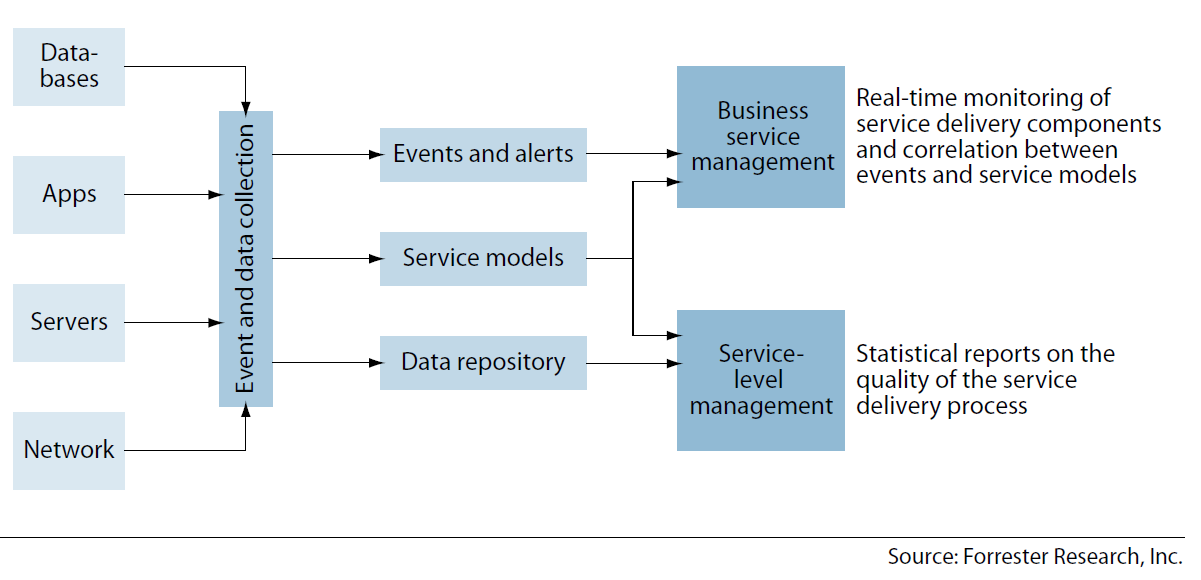
\includegraphics[scale=0.47]{biltli/forrester_bsm_slm.png}
\end{figure}

\section{Service Level Objectives (SLOs)}

SLAs werden als das Instrument betrachtet, durch welches der Dialog zwischen dem Kunden und dem Dienstleister etabliert werden kann. Die {\em Service-level objectives} (SLOs) wiederum sind dann die Parameter, mit welchen die Zufriedenheit über den angebotetenen Service gemessen wird \cite{forrester:slaBestPractices}. Gemäss Forrester funktioniert das aber nur, wenn folgendes gilt:

\begin{itemize}
\item Die SLOs werden genau dort gemessen, wo die Dienstleistung verwendet wird.
\item Die SLOs sind eine korrekte Repräsentation derjenigen Aspekte, die für den Kunden wichtig sind.
\end{itemize}

\section{Metriken}

Gemäss Forrester (\cite{forrester:slaBestPractices}) soll eine in einem SLA verwendete Metrik die folgenden Anforderungen erfüllen:

\begin{enumerate}
\item Die Metrik ist objektiv messbar.
\item Die Metrik enthält eine klare Aussage über das erwartete Resultat.
\item Die Metrik unterstützt Business-seitige Anforderungen.
\item Die Metrik konzentriert sich entweder auf die Effektivität oder die Effizienz des zu messenden Prozesses.
\item Die Metrik erlaubt eine sinnvolle statistische oder Trend-Analyse.
\item Die Metrik wendet Industrie- und/oder andere Standards an.
\item Annahmen und Definitionen für zufriedenstellende Performance wird spezifiziert.
\item In die Festlegung der Metrik wurden diejenigen Stakeholder involviert, die nachher für die Performance des Prozesses verantwortlich sind.
\item Sowohl der Dienstleister wie auch der Abnehmer akzeptieren die Metrik.
\end{enumerate}

\section{Key Performance Indications (KPIs)}

\section{Web Service Level Agreements (WSLAs)}

SOA (Service Oriented Architecture) ist ein aktuelles Buzzword: Innerhalb von Business-Prozessen agierende Applikationen, die sich dynamisch an ihre benötigten Services binden. Als Quasi-Standard haben sich in diesem Umfeld Web-Services durchgesetzt.

Die dafür notwendigen Definitionen sind mittlerweile ebenfalls standardisiert oder quasi-standardisiert:
\begin{description}
\item[SOAP] ein XML-basiertes Austauschformat für Messages \cite{wiki:soap}
\item[WSDL] ein XML-basiertes Austauschformat für Daten- und Operationen-Definitionen \cite{wiki:wsdl}
\end{description}

Für sinnvolles End-to-End-Monitoring der Business-Prozesse müssen natürlich auch die daran beteiligten Web-Services überwacht werden können -- und entsprechende SLAs zwischen dem Anbieter des Service (oder dem Service selbst) und dem Konsumenten vereinbart werden können.

Da die Benutzung von Web-Services aber dynamisch funktioniert (d.h. eine Fall-zu-Fall-Geschäftsbeziehung eingegangen wird), müssen schlussendlich auch Definition, Verhandlung, Festlegung, Überwachung und Durchsetzung der zugehörigen SLAs dynamisch (sprich automatisiert) funktionieren können \cite{ibm:wslaPaper}.

Klassische SLAs sind als Freitext formuliert -- was aus naheliegenden Gründen in direktem Widerspruch zur Anforderung der Automatisierbarkeit steht.

Die aktuelle Praxis (auch für alle anderen Arten von Agreements) ist darum, Templates zu entwickeln -- Freitext, welcher die grundlegenden Züge der Abmachung beschreibt, kombiniert mit semantischen Feldern. Dieser Ansatz hat allerdings das Problem, dass er einigermassen unflexibel und nur für sehr grundlegende SLOs genügend ist \cite{ibm:wslaPaper}.

Findige Köpfe von IBM haben darum 2003 dafür eine grundsätzliche Lösung vorgestellt: Das Web Service Level Agreement Framework \cite{ibm:wslaSpec, ibm:wslaPaper}, mit den folgenden Anforderungen und Design-Zielen:
\begin{description}
\item[Flexible formale Sprache, die einen weiten Bereich von SLAs abdeckt.] Es hat sich gezeigt, dass SLA-Parameter verschiedener Provider und unterschiedlicher Services, die identisch erscheinen, trotzdem stark in ihrer Semantik variieren. Darum ist es wichtig, dass ein SLA-Framework die Parteien nicht in der Formulierung der SLAs einschränkt. Handkehrum sind aber SLAs in ihrer Struktur stets identisch. Jedes SLA enthält:
\begin{itemize}
\item die involvierten Parteien,
\item die SLA-Parameter,
\item die Metriken, welche die Parameter vervollständigen,
\item den Algorithmus, mit welchem die SLA-Parameter berechnet werden,
\item die SLOs,
\item sowie die Massnahmen, die im Falle einer Verletzung eines oder mehrerer SLOs zu treffen sind.
\end{itemize}
\item[Möglichkeiten zur Integration mit eCommerce-Systemen und -Plattformen] Bezüglich eCommerce und B2B ist die Automatisierung schon sehr weit fortgeschritten -- ein SLA-Framework sollte also in seinen Grundzügen kompatibel zu dortigen existierenden Ansätzen sein. IBM sieht vor allem folgende Integrationsmöglichkeiten:
\begin{itemize}
\item Bewerbung und Verkauf von SLA-basierten Services,
\item Integration in elektronische Marktplätze wie jene von Ariba (welche mittlerweile von SAP übernommen worden ist \cite{wiki:ariba}) oder CommerceOne (welche mittlerweile konkurs gegangen ist \cite{wiki:commerceone}),
\item weitere Marketplace- und Matchmaking-Anwendungen \cite{Bichler200106}, auch für das Matching von Produkten mit komplexen Attributen (die eben in den SLAs spezifiziert werden können),
\item automatisierte Verhandlung, wie beispielsweise vom Projekt SilkRoad vorgesehen \cite{Strobel:2001:DRP:593916.593929, Stroebel00aframework},
\item Verknüpfung von Business-Prozessen über Organisationsgrenzen hinweg, beispielsweise über den ebXML-Stack \cite{wiki:ebxml, ibm:wslaPaper}
\end{itemize}
\item[Übertragung von Überwachungs-Verantwortlichkeiten an Drittparteien]
Die enhanced Telecom Operations Map (eTOM) \cite{ibm:wslaPaper, wiki:etom} definiert eine Vielzahl von Rollen, die ein Service-Provider einnehmen kann; und momentaner Stand der Dinge ist auch, dass ein SLA vor allem als bilaterales Abkommen zwischen zwei Parteien betrachtet wird. Es kann nun aber Fälle geben, in denen die Daten für die Metriken weder von der einen noch von der anderen Partei sinnvoll geliefert werden können. Ausserdem können Fälle auftreten, in denen die eine Partei der anderen in Bezug auf die korrekte Bereitstellung der Daten misstraut.

Aus diesem Grund definiert \cite{ibm:wslaPaper} diejenigen Parteien, welche das SLA tatsächlich unterschreiben (typischerweise der Dienstleister und der Kunde) als sogenannte {\em Signatory parties}, und lässt daneben eine beliebige Anzahl sogenannter {\em Supporting parties} zu. Diese übernehmen beispielsweise Messungen oder die Auswertung der Daten.
\item[{\em Need-to-know Principle} für das Deployment von SLAs]
Es liegt auf der Hand, dass alle SLA-relevanten Definitionen sowie alle Parteien (ob Signatory oder Supporting im Sinne von oben) in einem einzigen SLA festgelegt sein sollten. Gleichzeitig kann aber die Landschaft der involvierten Parteien einigermassen komplex werden -- und bestimmte Parteien werden das Bedürfnis haben, dass sie (oder Drittparteien) für andere nicht sichtbar sind.

Beispielsweise möchte ein Service Provider, der Teile (oder das Ganze) seines Services wiederum von einem dritten Service Provider einkauft, diesen nicht offenlegen. Des weiteren möchte wohl keine der Signatory parties den Supporting parties mehr Kennzahlen als nötig offenlegen (vor allem keine Preise) \cite{ibm:wslaPaper}.

Diese Anforderung macht das Deployment eines SLAs bei den verschiedenen involvierten Parteien einigermassen kompliziert, denn es dürfen nur diejenigen Teile ausgerollt werden, die jeweils notwendig sind, damit eine Partei ihre Rolle wahrnehmen kann.

Aus diesem Grund schlagen die Autoren von IBM einerseits einen speziellen Deploy\-ment-Service vor (dessen Einbettung in den Gesamtkontext der Abbildung \ref{wslacontext} entnommen werden kann), einerseits ein zweistufiges Deployment-Verfahren:
\begin{enumerate}
\item Der Deployment-Service generiert Konfigurationsinformation im sogenannten {\em Service Deployment Information (SDI)}-Format (\cite{ibm:wslaPaper, ibm:wslaSpec}) an die Supporting parties.
\item Die Supporting parties konfigurieren ihre eigenen Systeme anhand der Informationen im gesandten SDI.
\end{enumerate}
\item[SLA-getriebene Konfiguration von verwalteten Ressourcen]
Da die Etablierung eines SLAs weitreichende Konsequenzen auf die Konfiguration der verwalteten Ressourcen eines Service Providers haben kann, muss ein SLA-Management-Framework wie das besprochene die Möglichkeit bieten, einerseits sich auf bestehende Infrastruktur zu beziehen, andererseits die existierenden Metriken dieser existierenden Infrastruktur zu nutzen und zu den definierten Metriken innerhalb des SLAs in Beziehnung zu setzen. Beispielsweise existiert ein RFC für ein MIB für SLA-Performance-Messung in SNMP-Umfeldern \cite{ibm:wslaPaper, rfc2758}.
\end{description}

\begin{figure}
\caption{WSLA-Services und ihre Interaktionen}
\label{wslacontext}
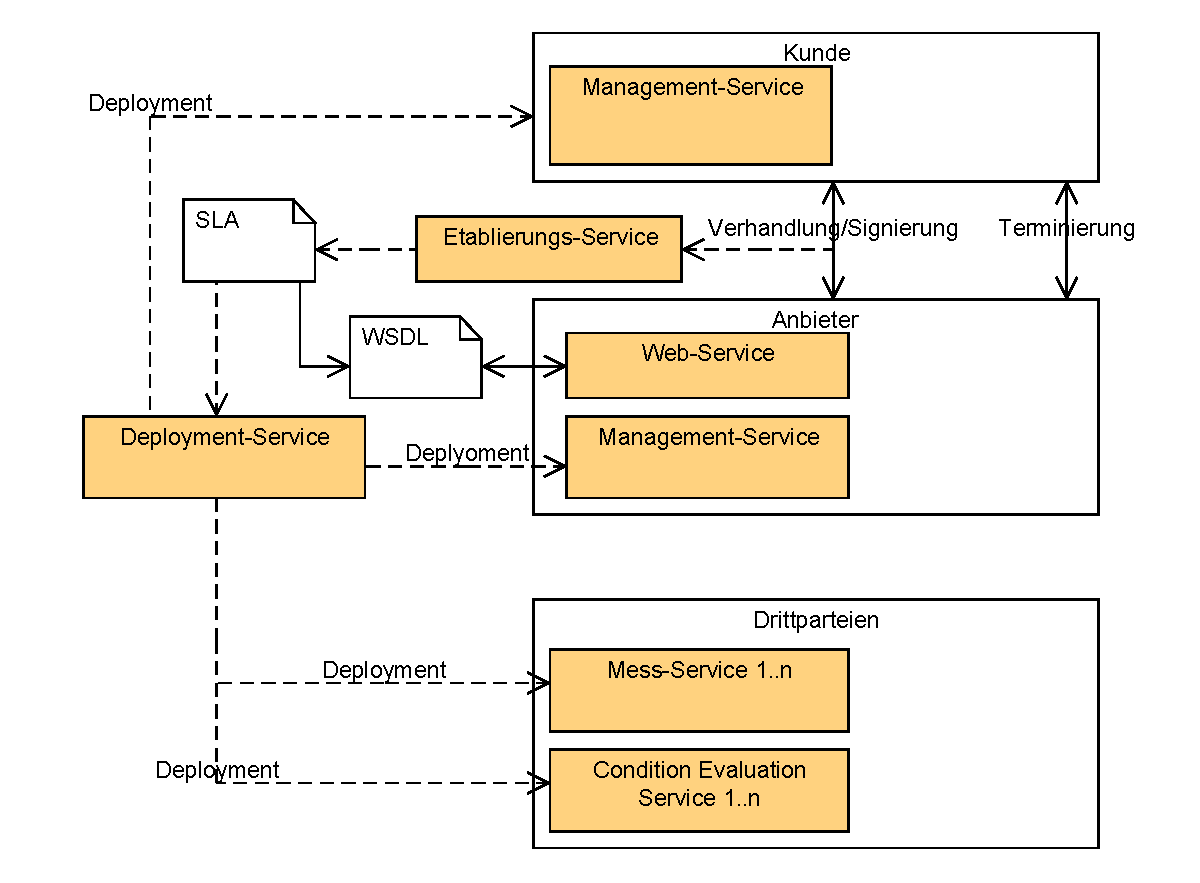
\includegraphics[scale=0.7]{diagramme/wsla_context.pdf}
\end{figure}

Alle diese Anforderungen führen zu entsprechenden Services und Sprachdefinitionen. Das grundsätzliche Schema ist in Abbildung \ref{wslaone} dargestellt. Die wesentlichen Komponenten sind die folgenden:

\begin{figure}
\caption{Eine 3-Parteien-WSLA-Konstruktion}
\label{wslaone}
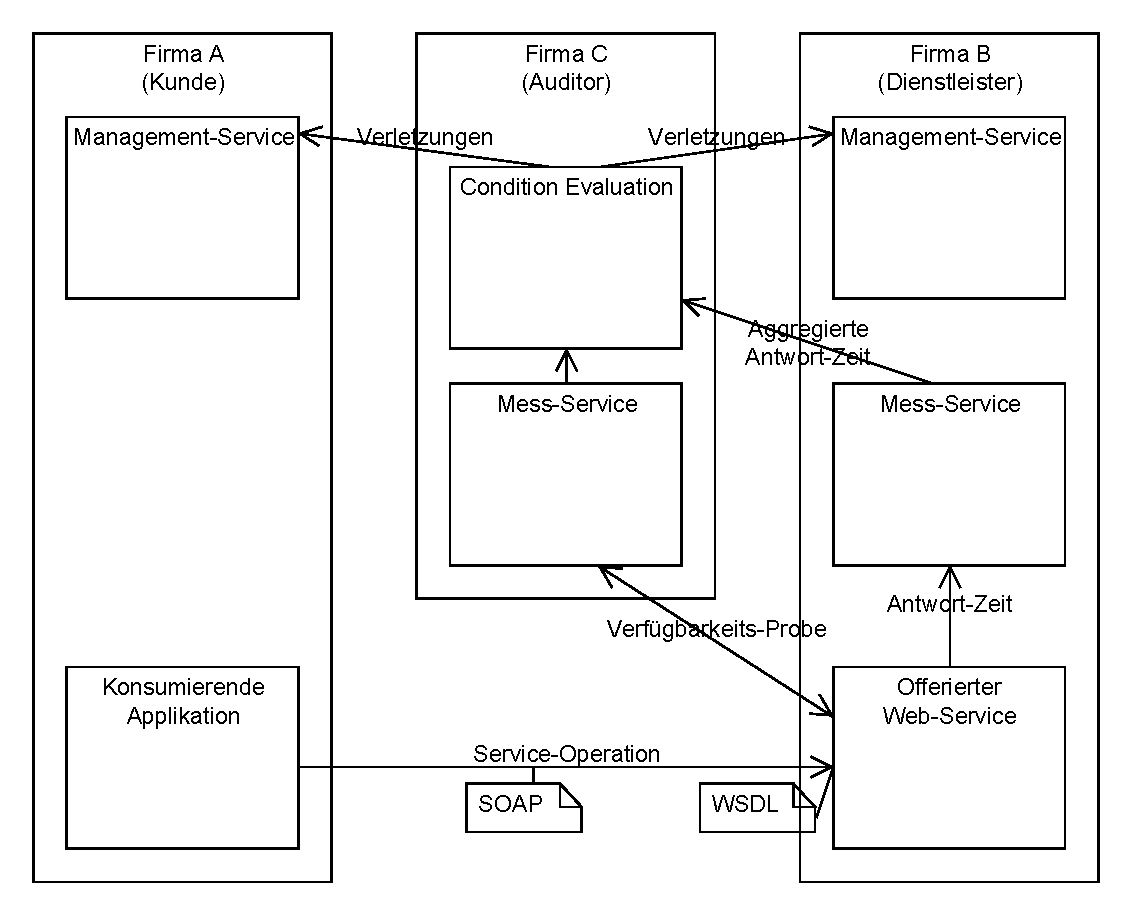
\includegraphics[scale=0.6]{diagramme/wsla_basic.pdf}
\end{figure}

\begin{description}
\item[Offerierter Web-Service] Der Web-Service, der zur Verfügung gestellt wird. Das WSLA dient primär der Überwachung dieses Services.
\item[Konsumierende Applikation] Die Applikation (oder Service oder Business-Prozess), welche den offerierten Web-Service konsumiert.
\item[Mess-Service innerhalb Firma B] Ein Service, welcher direkt durch Konsumation anfallende Metriken des offerierten Web-Services misst (beispielsweise die Antwort-Zeit).
\item[Mess-Service innerhalb Firma C] Ein Service, welcher indirekte und globale Metriken misst (beispielsweise, ob der Service überhaupt verfügbar ist).
\item[Condition Evaluation Service] Ein Service, welcher die Metriken der verschiedenen Mess-Services erhält und gegen den Inhalt des SLAs überprüft.
\item[Management-Service innerhalb Firma A] Ein Service, der Notifikationen über Verletzungen des SLAs erhält und darauf entsprechend reagiert.
\item[Management-Service innerhalb Firma B] Ein Service, der Notifikationen über Verletzungen des SLAs erhält und darauf entsprechend reagiert.
\end{description}

Die Sprache besteht aus folgenden drei Teilbereichen:
\begin{description}
\item[Parties] Dieser Bereich definiert alle in das SLA involvierten Parteien. 
\item[Service Description] Dieser Bereich spezifiziert die Charakteristika des Services und seine beobachtbaren Parameter \cite{ibm:wslaPaper}, welche für die Mess-Services von Bedeutung sind. Als Beispiel einer Service Description sei ein Service gemäss Abbildung \ref{wsladesc} gegeben. Die wesentlichen Elemente sind {\tt SLAParameter} und {\tt Metric} -- {\tt SLAParameter} definiert vor allem die Kommunikationseigenschaften (welche Party wird darüber informiert), während {\tt Metric} die dazugehörige Metrik mit einer Berechnungsfunktion sowie Referenzen auf darunterliegende Metriken enthält. Die XML-Listings in den Abbildungen \ref{wslaparamxml} und \ref{wslametricxml} sollen dies illustrieren.

\begin{figure}
\caption{Beispiel für eine WSLA-Service Description}
\label{wsladesc}
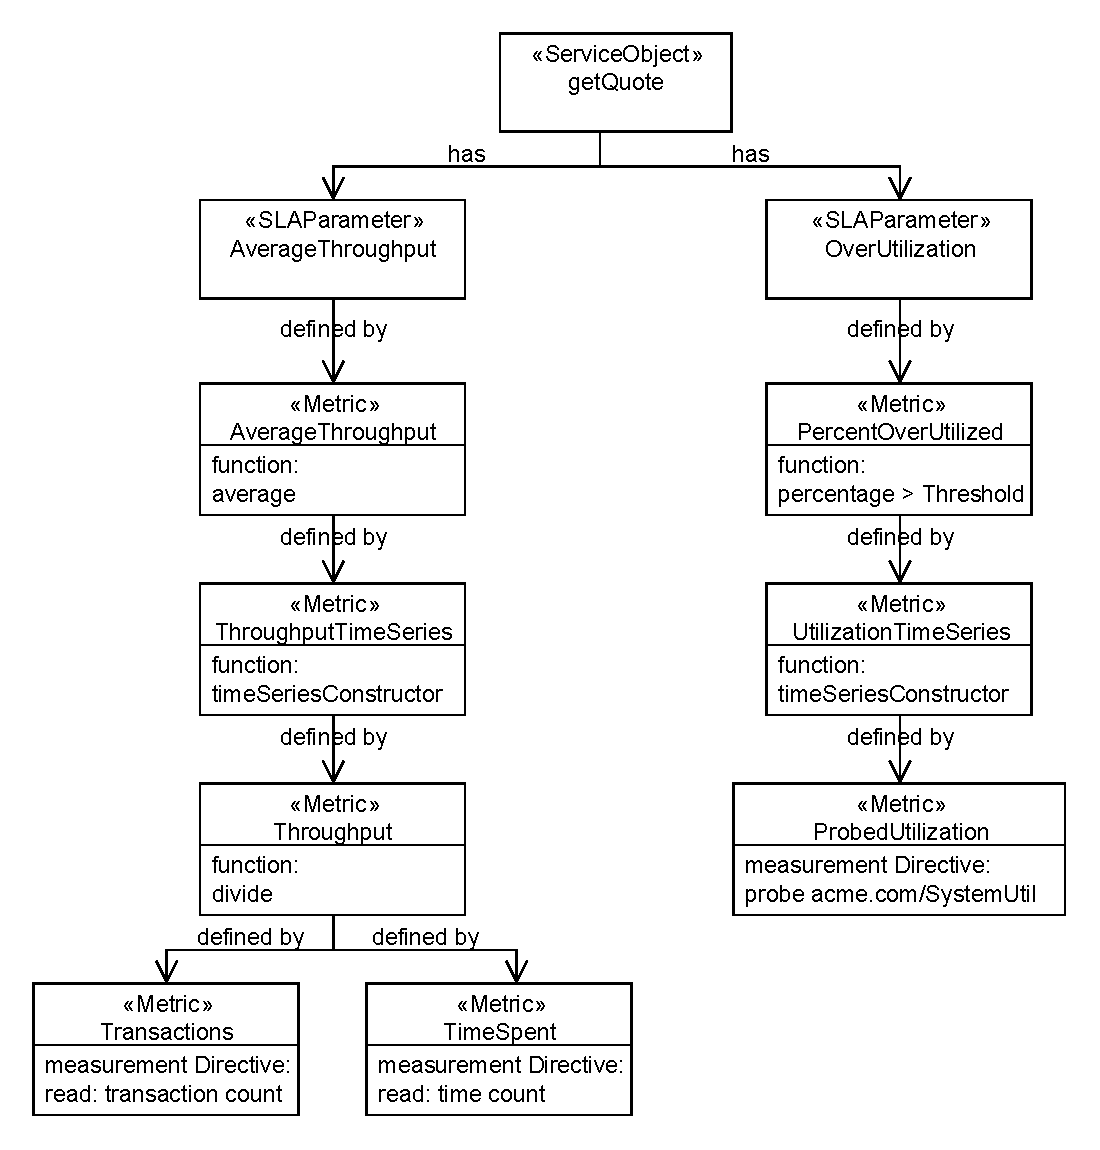
\includegraphics[scale=0.6]{diagramme/wsla_servicedesc.pdf}
\end{figure}

\begin{figure}
\caption{XML-Definition eines WSLA-{\tt SLAParameter}}
\label{wslaparamxml}
\begin{lstlisting}
<SLAParameter name="OverUtilization" type="float" unit="Percentage">
	<Metric>PercentOverUtilized</Metric>
	<Communication>
		<Source>Firma B</Source>
		<Pull>Firma C</Pull>
		<Push>Firma C</Push>
	</Communication>
</SLAParameter>
\end{lstlisting}
\end{figure}

\begin{figure}
\caption{XML-Definition einer WSLA-{\tt Metric}}
\label{wslametricxml}
\begin{lstlisting}
<Metric name="PercentOverUtilized" type="float" unit="Percentage">
	<Source>Firma C</Source>
	<Function xsi:type="percentage > Threshold" resultType="float">
		<Schedule>BusinessDay</Schedule>
		<Metric>UtilizationTimeSeries</Metric>
		<Value>
			<LongScalar>0.8</LongScalar>
		</Value>
	</Function>
</Metric>

<Metric name="UtilizationTimeSeries" type="TS" unit="">
	<Source>Firma C</Source>
	<Function xsi:type="timeSeriesConstructor" resultType="float">
		<Schedule>Every5Minutes</Schedule>
		<Metric>ProbedUtilization</Metric>
		<Window>12</Window>
	</Function>
</Metric>

<Metric name="ProbedUtilization" type="float" unit="">
	<Source>Firma B</Source>
	<MeasurementDirective xsi:type="Gauge" resultType="float">
		<RequrestURL>http://acme.com/SystemUtil</RequestURL>
	</MeasurementDirective>
</Metric>
\end{lstlisting}
\end{figure}

\item[Obligations] Dieser Bereich spezifiziert diverse Garantien und Einschränkungen, welche für SLA-Parameter gegeben werden können. Dieser Bereich ist vor allem für den Condition-Evaluation-Service von Bedeutung.
\end{description}

\section{Gestaltung von IT-Leistungskatalogen mit E2E}

\section{Outsourcing: Auswirkungen von E2E}

Die Weiterentwicklung der Fähigkeiten der IT im Generellen hat viele neue Möglichkeiten gebracht, wie IT das Business direkt unterstützen und zur Wertschöpfungskette beitragen kann. Gemäss Forrester (\cite{forrester:slaBestPractices}) zeitigen sich daraus allerdings zwei sich widersprechende Effekte:

\begin{description}
\item[Die IT-Abhängigkeit des Business nimmt zu.] Praktisch sämtliche Unternehmen haben einen Punkt erreicht, an dem ihre Business-Prozesse so abhängig von einer funktionierenden IT sind wie von Elektrizät und fliessendem Wasser.
\item[Der Kostendruck auf die IT nimmt zu.] Externe Dienstleister haben für die Mehrheit der IT-Geschäftsfelder Lösungen entwickelt, die direkt mit den Dienstleistungen der internen IT-Abteilungen konkurrenzieren können. Gemäss der Logik des Marktes resultieren daraus sinkende Preise und steigende Qualität.
\end{description}

Die interne IT kann sich nun entweder dieses Konkurrenz- und Kostendrucks annehmen, sich auf den Einkauf von externen Services und deren Weitervermittlung an das Business konzentrieren, oder eine Mischform der ersten beiden anstreben.

Alle drei Strategien setzen aber voraus, dass die IT ihre operationelle Struktur derer eines IT-Dienstleisters angleicht. Dafür braucht sie entsprechendes Qualitätsmanagement, um dem Business ihren Wert beweisen zu können.

\chapter{Fazit}

\listoffigures

\bibliography{Referenzen}
\bibliographystyle{plain}

\end{document}
